\documentclass{template/template}

%\renewcommand{\familydefault}{\sfdefault} %% Only if the base font of the document is to be sans serif
%\usepackage{bera}

\usepackage[T1]{fontenc} % evropské uvozovky
\usepackage{subcaption}
\usepackage{amsmath}
\usepackage{enumitem}
\usepackage{hyperref}
\usepackage{gensymb} % balíček symbolů
\usepackage{booktabs}
%\usepackage{lmodern}
\usepackage{csquotes} % text lze uvést do uvozovek pomocí \enquote{text}
\usepackage{textcomp}

\usepackage[toc,page]{appendix}
\usepackage{color} % balíček pro obarvování textů
\usepackage{xcolor}  % zapne možnost používání barev, mj. pro \definecolor
\definecolor{mygreen}{RGB}{0,153,153} % nastavení barev odkazů 
\definecolor{myblue}{RGB}{0,0,200} 
\definecolor{commentgreen}{RGB}{0,100,0} % nastavení barev pro příklady z C++
\definecolor{deepblue}{rgb}{0,0,0.7}
\definecolor{deepred}{rgb}{0.6,0,0}
\definecolor{deepgreen}{rgb}{0,0.5,0}
\usepackage{listings} % balíček pro formátování zdrojových kódů 
\usepackage[author=,status=draft]{fixme} % vkládání poznámek  
% dva módy (status): draft (poznámky se zobrazují v PDF) / final (poznámky se nezobrazují v PDF)
\usepackage{graphicx}
\usepackage{multirow}
\usepackage{float}


\usepackage[T1]{fontenc} % import tučného písma typu tt pro prostředí listings
%\usepackage{listings} % balíček pro obarvování syntaxe ukázek programů v textu
\usepackage{listingsutf8} %nutné pro \usepackage{listings} aby to jelo v UTF-8
\lstset{
	extendedchars 	= false,
	language      	= C++,
	basicstyle      = \ttfamily,
	keywordstyle     = \bfseries,
	%identifierstyle = \color{brown},
	commentstyle    = \color{commentgreen},
	otherkeywords	= {self},             % Add keywords here
	emphstyle		= \color{deepred},    % Custom highlighting style
	stringstyle	 	= \color{deepgreen},		
	keywordstyle	=\color{deepblue},
	stringstyle     = \color{magenta},
} % písmo a  barvičky  by možná chtěly doladit - nějaký dobrovolník? 
% volba literate= pro znaky s diakritikou z kódů se zvýrazněnou syntaxí se nesmí používat, rozbíjí překlad

% \begin{lstlisting} Tady je zdrojový kód např. v C++ \end{lstlisting} - pro UTF-8 NE
%\lstinputlisting{source_filename.py} vloží soubor z daného místa a obarví

\usepackage{hyperref} % balíček pro hypertextové odkazy
% \url{www.odkaz.cz}
% \href{http://www.odkaz.cz}{Text který bude jako odkaz}
%\hyperlink{label}{proklikávací_text} - odkaz na text 
% \hypertarget{label}{cíl_odkazu} - cíl odkazu  


\hypersetup{colorlinks=true, linkcolor=myblue, urlcolor=mygreen, citecolor=blue, anchorcolor = magenta,
	linktocpage = true, frenchlinks } % nastavení barvy odkazů 
% bookmarksopen=true, bookmarksnumbered=true, bookmarksopenlevel=1 - nastavuje rozbalování levého menu       





%\usepackage{expl3} % bibtex dependency, must be loaded prior to the bibtex
%\usepackage[backend=bibtex,bibstyle=numeric,sorting=none,date=long,dateabbrev=false,texencoding=utf8,bibencoding=utf8,style=iso-numeric]{biblatex}

\usepackage[a4paper]{geometry}

%\lstset { 
%    language=C++,
%    backgroundcolor=\color{black!5}, % set backgroundcolor
%    basicstyle=\footnotesize,% basic font setting
%}

%\addbibresource{text.bib}
%\nocite{*}

\titlecz{Párty světla} % Název práce
\author{Anna Králová} % Jméno autora
\institution{STŘEDNÍ PRŮMYSLOVÁ A~VYŠŠÍ ODBORNÁ ŠKOLA BRNO, Sokolská 1} % Celý název instituce
\institutiontype{příspěvková organizace} % Typ instituce
\thesistype{Ročníková práce}  % Typ práce/dokumentu
\mentor{Mgr. Miroslav Burda} % Jméno vedoucího práce
%\mentorstatement{Ing. Václava Zavadila} % Jméno vedoucího práce ve čtvrtém pádě

% Newly added
\authorname{Anna}
\authorsurname{Králová}
\schoolyear{2020/2021}
\field{Technické Lyceum} % Studijní obor
\class{L3A}

\placefooter{Brno 2021}

% \usepackage{hyperref} % balíček pro hypertextové odkazy
% \url{www.odkaz.cz}
% \href{http://www.odkaz.cz}{Text který bude jako odkaz}
% \hyperlink{label}{proklikávací_text} - odkaz na text 
% \hypertarget{label}{cíl_odkazu} - cíl odkazu 

%%% Přepínač pracovní kopie
\workcopytrue
%\workcopyfalse

%\renewcommand\bibname{Literatura a zdroje}

\begin{document}
\hyphenation{SOLIDWORKS Solid/-Works}

\newgeometry{margin=2cm, top=3cm, bottom=2.5cm, left=2.5cm, includefoot}

\maketitle

\newgeometry{margin=2cm, top=2.5cm, bottom=2.5cm, left=2.5cm, right=2cm, includefoot}

\makecopyrightstatement{V~Brně}



\pagestyle{empty}

\section*{Zadání}

Cílem této ročníkové práce je sestrojit fukční prototyp malého světýlka za použití programovatelného, inteligentního LED Pásku. 


%\subsection*

\vspace{20mm}

%\section*

%\subsection*

\newpage
\pagestyle{plain}

\tableofcontents % vysází obsah

\setlength{\parskip}{0.4em}

%%% Začátek práce
\setcounter{figure}{0}
\setcounter{table}{0}
\newpage

% Úvod práce
\chapter*{Úvod}
\addcontentsline{toc}{chapter}{Úvod}

 %(viz kapitola \ref{3_kap}).
Každý z nás má rád malé dekorace. Ať už jsou to malé sošky, které pokládáme na poličky v našich pokojích, nebo obrovské vázy, či kusy drúz na ozdobení našich obývacích pokojů. Dekorace ale nemusí být jen takto jednoduchá. Občas se může jednat i o lampičky roztodivných tvarů, nebo vodní mlýnky, které v sobě mají zabudované LED a pomocí cirkulující vody se paprsky světla lámou dopadají na stěnu, což by se dalo nazvat dekorací samo o sobě.
%\cite{schommers}

Mě osobně se vždycky líbily malé průhledné stromečky, které se prodávaly na Vánoce a~jejich barva se postupně měnila. A tak mě napadlo, proč něco takového také nevyrobit, ale tentokrát místo stromečku použít tvar nějaké květiny, která by měnila barvu světla podle ovládání. %(viz kapitola \ref{3_kap}).


Cílem této ročníkové práce je sestrojit prototyp takového dekoračního světla, včetně naprogramování inteligentního LED pásku, dokumentace a možných návrhů, jak tento nápad inovovat.
%\href{https://www.tecomat.cz/products/}{teco}

%todo zadání

%todo odkaz na knihovny

%todo (viz kapitola \ref{3}) --> otázka na učitele?


%Vložíme podle návodu autora programu
%moduluje wifina
%V módech světla -- reference na poslední kapitolu
%Vytvořit na Githubu sloéžku pro původní program, který jsem poté upravila
%přidat subchapters do 4. a 5. kapitoly
%Pájení --> obrázek zapájené soustavy DevKitC a LED 
%Rozepsání se, co je Visual Studio Code Zač
%Propagace letního robotického tábora

%Odkazy? Github?


% Proč?
\chapter{Použité součástky}

V této kapitole budou představeny součástky, se kterými se v budoucnu použijeme

\section{ESP32 DevkitC}
%Co to je?
ESP32-DevKitC je malá programovatelná deska založená na ESP32 od společnosti Espressif. Vstupní a výstupní piny se nachází na obou stranách desky, což umožňuje uživateli připoji periferní zařízení jak pomocí propojovacích vodičů, tak připojením k nepájivému poli. Na desce se také nachází mikro-USB port který dovoluje  desku jedoduše napájet přímo z počítače, stejně jako nahrávat na desku soubory. 

\begin{figure}[htbp]
	\centering
	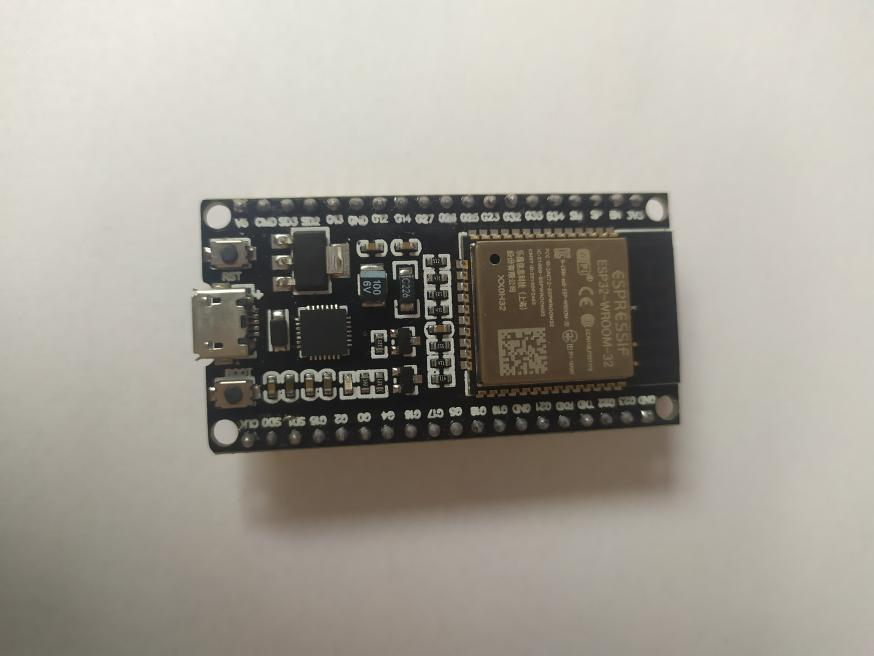
\includegraphics[width=0.7\textwidth]{img/ESPDevKit.jpg}
	\caption{ESPDevKit}
	%	\label{fig:install-sdk-3}
\end{figure}

%Co se s tím dá dělat
Deska je pompatibilní s Arduinem a často se v kombinaci zrovna s tímto typem součástek používá. Díky zabudovanému Wifi modulu je možné se na součástku napojit a používat jakékoliv zařízení pracující s Wifi, (například chytrý mobil), aby se k součástce napojilo a fungovalo jako dálkový ovladač, což jsem v praxi nejčastěji viděla už ke zvýše zmíněnému programování LED světel, ale prakticky se s ESP32 DevkitC dá dělat prakticky cokoliv: Použít ho jako procesor pro po domácku vyrobený alarm, nebo zaznamenávaše počasí. 


%Proč jsem si vybrala zrovna tuto součástku.
Já se ESP32 DevkitC rozhodla použít nejen proto, že v mém okolí mělo spoustu lidí s touto technoligií zkušenosti a mohli mi v případě nějakého problému jednoduše pomoct, ale hlavně kvůli dostupnosti a všestranému využití. Navíc Wifi modul na této desce se jednoduše dá využít pro dálkové ovládání ESP32 z mobilu což vyhovuje našim záměrům. Navíc rozměry desky ESP32 DevkitC(přibližně 5,5 cm na 3 cm) jsou vyhovující pro pozdější vybudování napájecí základny, která bude napájet a řídit LEDky schované v průchledném plastové květině.



\section{NeoPixel modul s 8 RGB LED WS2812}
%Co to je? Co se s tím dá dělat
Jedná se o pevný pásek s inteligentními LED diodami za sebou. Často využívá jako výstupní model pro Arduino a obsahuje 8 RGB LED diod typu WS2812, kterou lze najít i pod označením NeoPixel. Výhoda tohoto LED pásku je, že se dá řídit pomocí jednoho datového pinu a dvěma napájecími piny, což umožňuje kontrolér ve WS diodách. Tento modul se sice nehodí našemu původnímu záměru, který vyžaduje, ale Ledky byli na pásku ohebném, ale jako modul pro testování postačí.

\begin{figure}[htbp]
	\centering
	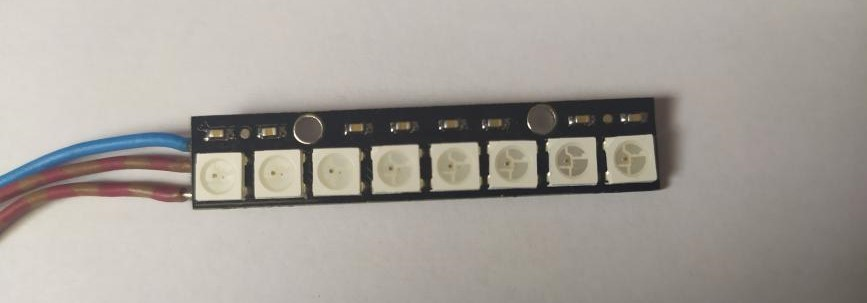
\includegraphics[width=0.7\textwidth]{img/NeoPixel2.jpg}
	\caption{NeoPixel}
	%	\label{fig:install-sdk-3}
\end{figure}

%Proč jsem si vybrala zrovna tuto součástku.
Tuto součástku jsem se rozhodla použít ze dvou důvodů. Ten první byl, že jsem neměla ještě úplně jistě vybraný finální ohebný led pásek, jaký bych chtěla použít. Ten druhý důvod byl stejně, jako v případě ESP, že kdyby nastaly při práci s tímto modulem nějaké problémy, tak jsem znala spoustu lidí, kteří by mi s případnými problémy dokázali pomoci. 


\section{Pásek ws2812 ohebný}
Po nějaké době práce s předchozím LED-páskem jsem si nakonec rozhodla vybrat skoro totožný pásek až na určitou maličkost, a to, aby byl Jednoduše ohebný a tvarovatelný. Pracuje a programuje se s ním stejně, jako s předchozím páskem, avšak, jelikož to více vyhovovalo záměru tak jsem tentokrát použila pásek se čtyřmi RGB LED diodami. 


\begin{figure}[htbp]
	\centering
	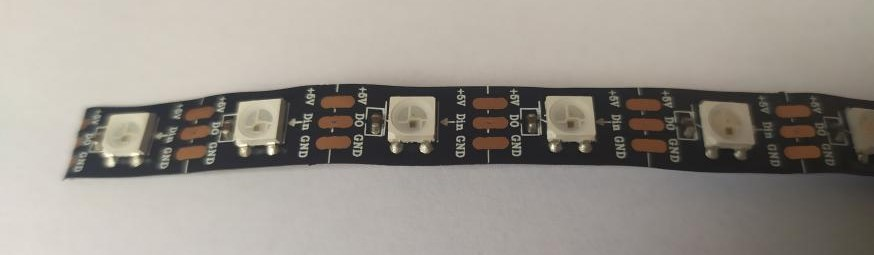
\includegraphics[width=0.7\textwidth]{img/OhebnyLedPasek2.jpg}
	\caption{{Pásek ws2812}
	%	\label{fig:install-sdk-3}
\end{figure}


\section{Pájení}

Proto, abych s těmito součástkami mohla dál pracovat, potřebovala jsem napojit Pevný LED NeoPixel pásek na ESPDevKit. Což jsem udělala tak, že jsem k Neopixel pásku připájela dráty na kontakty: napájení, uzemění a vstupní pin. Na tyto dráy jsem z druhé strany přidělala ((Ta černá koncovka která nevím jak se jmenuje)) a napojila jsem je z druhé strany na ESPDevKit. Jako vstupní pin jsem zvolila pin č. 21.  


%Otázky na učitele:
%Mám přidat obrázky? 
%Nevím jak pojmenávávat jednotlivé komponenty. Stačí to takhle? 

%Ostatní poznámky:
%Deska má tři druhy napájení, ale já budu využívat pouze napájení zkrz mikro-USB protože je to pro mě nejjednodušší. Stejně tak do toho budu posílat nahrané soubory z počítače
%Je potřeba vymyslet systém napájení
%Jak to funguje? Jaké je rozložení dané desky? 


% Realizace projektu
\chapter{Program}

\section{V čem psát program a jeho tvorba}

Pro psaní kódu jsem použila školní knihovny na programovaní LED světel, které byly původně vyrobeny pro Letní Robotický Tábor od 
 \href{https://helceletka.cz/tabory/#id=5357}{Helceltky}. Měla jsem tak o něco lehčí práci, protože jsem knihovny nemusela vytvářet sama. Program jsem se rozhodla psát v programu Visual StudioCode,\cite{Visualstudio} což je bezplatný editor zdrojového kódu, používající se také na víše zmíněném Letním Robotickém táboře pro práci zrovna s těmito knihovnami. Já pracovala s~Visual Studio Code již v minulosti, a i zde platilo, že jsem kolem měla lidi, kteří mi pomohli ve chvíli, když jsem měla s něčím problém. 

Začátek mého programu vypadal takto:

%todo odkaz na školní knihovny


%\href{https://www.tecomat.cz/products/}{teco}

%\lstinputlisting{priklady_c/blikani_LED1.cpp}
\lstinputlisting{Code/Zacatek-programu.cpp}


První dva řádky jsou knihovny, které jsem při psaní využívala. Další tři jsou definované proměnné, které určují, kolik LED světel pásek má (8), jaký pin zajišťuje komunikaci s~ESP32-DevKit (21), a číslo, které určuje, jaké číslo ponese první LED světlo s tím, že další LED byly očíslovány vzestupně.

%todo Otázka -->Odkazy na čtyři módy na github? 
\newpage

\section{První mód světla}
První barvu 
 \href{https://github.com/Nemesis-Rain/Supplements-/blob/main/4-barevne-mody/blikani-jedna.cpp}{prvního módu} jsem se rozhodla, že bude červená. Jen obyčejná červená bez jakýkoliv jiných barev nebo blikání. Nejdříve jsem ale musela nadefinovat funkci, která mi pomohla v dalším postupu a usnadnila mi manipulaci se všemi LED. 

%\lstinputlisting{priklady_c/blikani_LED1.cpp}
\lstinputlisting{Code/program1.cpp}


Nejdříve jsem si nadefinovala funkci \emph{SetLEDAll}, která mi při použití určitého příkazu, jak se LED mají rozsvítit, aplikovala tento příkaz na všechny LED na pásku, a umožnila mi jednodušší manipulaci s programem v pozdější fázi, když jsem všechny tyto módy přepisovala do jednoho programu. 
V kontextu tohoto programu to znamenalo, že když jsem barvu nastavila na červenou, zavolala se tato funkce a všechny LED se nastavili na stejnou, tlumeně červenou barvu. Tlumeně červenou proto, že LED zářily opravdu intenzivně a při jasu na 255 mě z nich začaly bolet oči. Proto jsem jas červené nechala na pouhé čtvrtině toho, co by LED zvládly.

%Funkce ShowLeds v sobě zase obsahovala dva příkazy, které se v programu nacházeli pro stabilizaci LEDek. 


\section{Druhý mód světla}
%nechci aby to blikalo jako blázen 
Jako \href{https://github.com/Nemesis-Rain/Supplements-/blob/main/4-barevne-mody/blikani-dva.cpp}{druhý mód} světla jsem se rozhodla, že použiju světle modrou barvu, která se bude pomalu stupňovat a pak tlumit a vznikne efekt pulzujícího modrého světla. Tohoto výsledku jsem docílila pomocí programu: 

%\href{https://www.tecomat.cz/products/}{teco}

%\lstinputlisting{priklady_c/blikani_LED1.cpp}
\lstinputlisting{Code/program2.cpp}

Tento program je navrhnut tak, že se zhasnuté LED začnou pomalu rozsvěcovat do jasné modré a poté znovu zhasínat do naprosté tmy. A jelikož byl tento příkaz napsán v části \emph{loop}, tento cyklus se bude opakovat do té doby, dokud nebude zavolána jiná funkce, nebo nebude \emph{ESP32-DevkitC} odpojena. Docílí se tak moc pěkného pulzujícího modrého efektu. 

Opět zde není použita plná síla LED světel, aby byly šetřeny moje oči.  

\section{Třetí mód světla}
Nápad na to, jak udělat pomalu pulzující světlo, mi připadal opravdu skvělý. Takže jsem se rozhodla něco podobného aplikovat i na \href{https://github.com/Nemesis-Rain/Supplements-/blob/main/4-barevne-mody/blikani-tri.cpp}{třetí mód}. Tentokrát jsem ale zkusila, jaké by to bylo, kdyby červená barva pomalu přešla do žluté a ze žluté do zelené a pak zase zpět.
%Trénovala jsem si tu přechod barev


%\lstinputlisting{priklady_c/blikani_LED1.cpp}
\lstinputlisting{Code/program3.cpp}

Program na tenhle mód je hodně jednoduchý a využívá podobného principu jako druhý mód. Opět tu je zpoždění, aby světlo bláznivě neblikalo. Původně jsem chtěla, aby barva připomínala oheň, což mi moc nevyšlo ale i tak to je moc pěkný přechod barvy, který při umístění do plastového krystalu nebo růže (něco jako \emph{žárovky}) vytvoří nádherný efekt. 
%todo Reference na poslední kapitolu? 

\section{Čtvrtý mód světla}
Původně jsem víc, než tři módy na LED neplánovala, ale po hraní si s různými barvami a~barevnými světelnými přechody jsem neodolala a přidala jsem do paměti ještě jeden \href{https://github.com/Nemesis-Rain/Supplements-/blob/main/4-barevne-mody/blikani-ctyri(duha).cpp}{čtvrtý mód}, který jsem pojmenovala \emph{Duha}.

%nevím co s tímto obrázkem. Jak udělat aby šel text hned vedle obrázku? 
%\href{https://www.tecomat.cz/products/}{teco}

%\lstinputlisting{priklady_c/blikani_LED1.cpp}
\lstinputlisting{Code/program4.cpp}


V podstatě na tomto programu není vůbec nic nového. Zase začíná na červené, kdy pomalu projde přes žlutou k zelené, dále pokračuje na světle modrou a tmavě modrou, až~se dostane z fialové a z fialové zpátky na začátek, což znamená na červenou. Tenhle efekt vypadá moc pěkně a vážně se pro barevné lampičky hodí. 


%Obrázky kódu? 
%Název školních knihoven nebo nějaká bližší specifikace? Kde se dají sehnat a stáhnout? 
%nevím jakým způsobem napsat zmínění knihoven
%const int CHANNEL = 0;???


% Návody na instalaci a rozjetí SolidWorks
\chapter{Ovládání přes mobil}
%Nemám nejmenší tušení co jsem psát, protože o té webovce nic, ale vůůůůůbec nic nevím


\section{Esp32-RBGridUI-Designer} %todo obrázek není tam, kde by měl být
Pro vytvoření ovládacího prostředí na mobilu, jsem použila {RBGridUI-Designer}, \cite{robotárna} což je prostředí vyvinuté přímo Robotárnou,\cite{robotárna} pro práci s LED a jejich ovládání přes mobil. Webová stránka {\em Esp32-RBGridUI-Designer} má toto rozložení: 
%todo Na následujícím obrázku lze vidět rozložení webové stránky se kterou jsem pracovala?
%todo předělat obrázek
\begin{figure}[htbp]
	\centering
	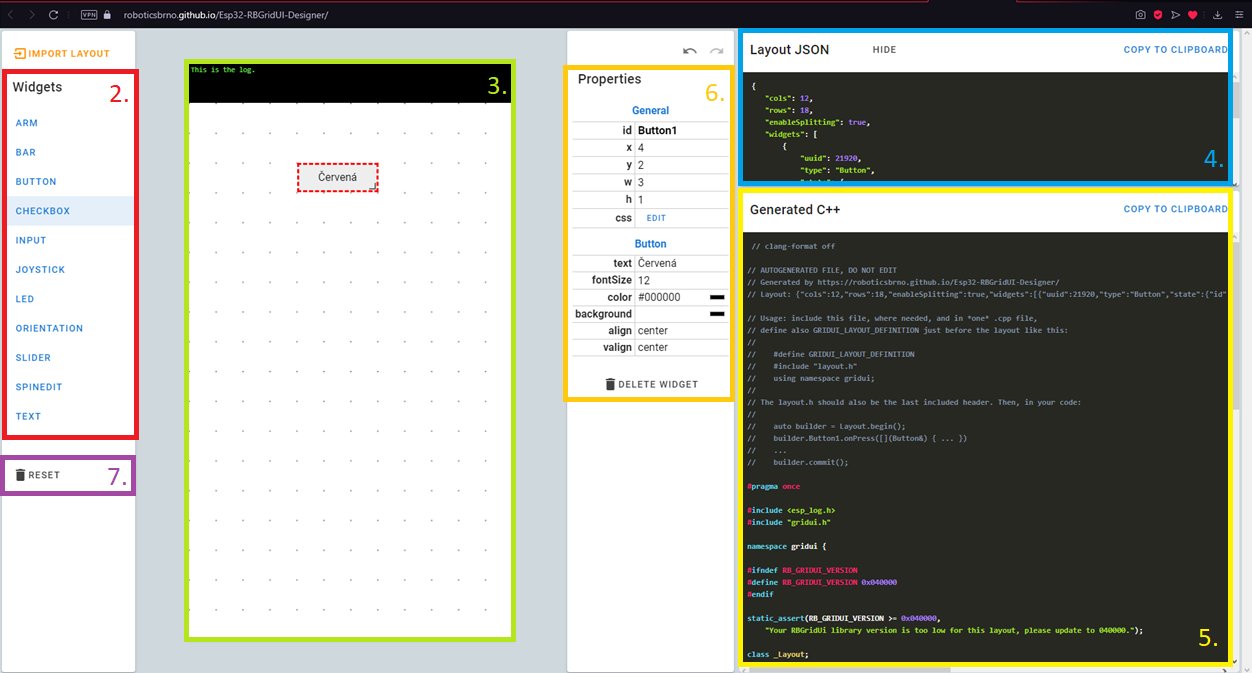
\includegraphics[width=1\textwidth]{img/Esp32-RBGridUI-Designer - malování.png}
	\caption{Prostředí stránky}
	%	\label{fig:install-sdk-3}
\end{figure}

\begin{enumerate}
	\item Postraní lišta, pri kliknutí na jakoukoliv komponentu, je uživatel schopen danou kamponentu přetáhnout na manipulační plochu
	\item Manipulační plocha, přetahují se sem tlačítka a nastavuje se jejich poloha a umístění, určuje vzhled řídící plochy v mobilu po stáhnutí aplikace
	\item Soubor, který je potřeba stáhnout a nahrát do stejné složky jako máme {/bf program}, nese informace toho, jakým způsobem jsme nanesli komponenty na manipulační plochu.
	\item /bf Něco %todo vysvětlit
	\item Bližší specifikace, určující umístění, barvu, a název tlačítka, které bylo vytvořeno na manipulační ploše. 
	\item Tlačítko Reset které vymaže veškeré komponenty z Manipulační plochy
\end{enumerate}


{\em Esp32-RBGridUI-Designer} je propojený s aplikací RBControler, \cite{RBControler}
%todo reference
\section{Vytvoření tlačítek}
Teď přišel čas na to, abych si připravila vlastní tlačítka. Každé tlačítko zpustí jiný mód, a ještě jsem tam chtěla mít tlačítko na vypnutí, takže jsem si celkově nadefinovala 5 tlačítek a pojmenovala je tak, abych se v jejich barvách vyznala. A poté jsem klikla na tlačítko copy to clipboad a zkopírovala jsem celý layout to textového souboru do stejné složky, jako jsem měla nový program  
%todoDalší obrázky aby to bylo pochopitelné?

\begin{figure}[htbp]
	\centering
	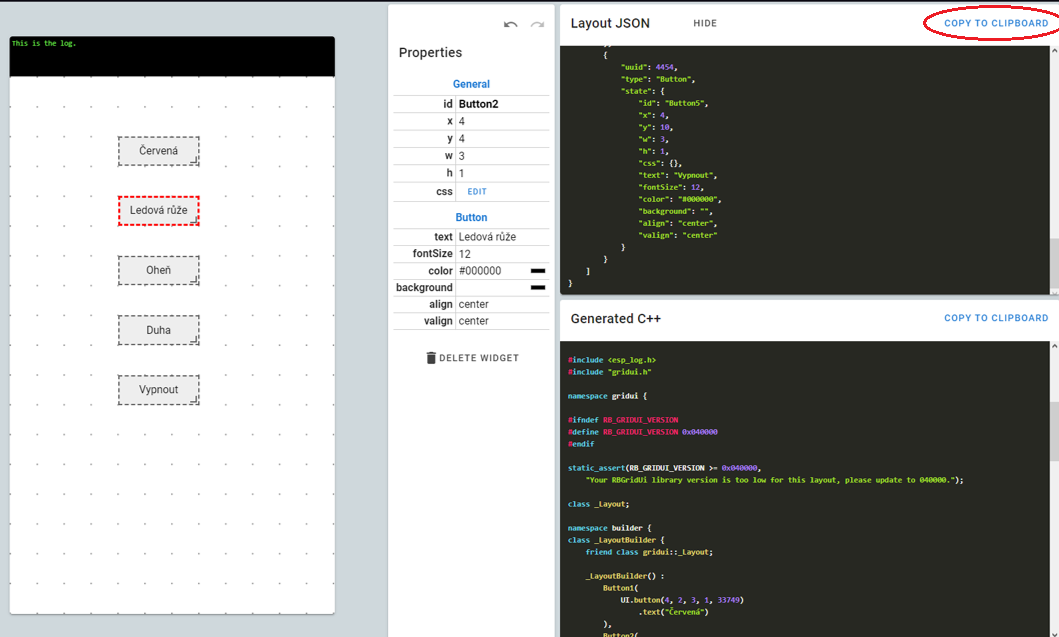
\includegraphics[width=0.8\textwidth]{img/Esp32-RBGridUI-Designer - Tlačítka.png}
	\caption{Tlačítka}
	%	\label{fig:install-sdk-3}
\end{figure}
%sooooo messy...
\section{Nový program} %todo Předělat celý tento odstavec
%todo Vyřešit/předělat nahrání programů?
Pro to, aby Ledky byli kompatibilní s programem, jsem si musela upravit jeden program který jsem dostala a který mi na mobilu fungoval. % todo odkaz na github 
Funkce void Setup() v následujícím programu ukazuje část nastavení mobilu a pak definování tlačítek a jejich funkcí. Funkce void Loop() dokončuje ukázku definování tlačítek, která je provedená pomocí funkce switch
%todo Reference na kapitolu
*Odkaz na Github*

\lstinputlisting{Code/new-program - Setup.cpp}

\lstinputlisting{Code/new-program - Loop.cpp}

\section{Propojení mobilu a ESP32-DevkitC a kontrola funkčnosti}
První krok byl, že jsem si stáhla aplikaci z Google play jménem RB Controler %todo odkaz
Poté jsem zapojila ESP32-DevkitC, ověřila jsem si, že je v něm nahraný konečný program a připojila jsem se na wifinu jménem LEDLED. 

%todo Zde bude screenshot obrazovky mého mobilu. (Wifi + ovládací panel)

Teď už jenom chtělo vyzkoušet, jak moc je daný program kompatibilní a funkční. %todo odkaz na video?

\newpage


% Modelování základních stroj.  součástí
\input{CHAPTERS/020 - FUNKČNOST LED.tex}

% Operace v sestavách
\chapter{Další možné využití}





%   \begin{figure}[htbp]
%	\centering
%	\begin{minipage}[b]{0.5\textwidth}
%		\centering
%		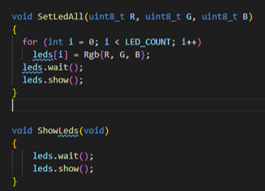
\includegraphics[width=0.75\textwidth]{img/015 img/definovane-funkce.png}
%		\caption{Funkce}
%		%		\label{fig:gear-sketch1}
%	\end{minipage}
%	\qquad
%	\begin{minipage}[b]{0.4\textwidth}
%		\centering
%		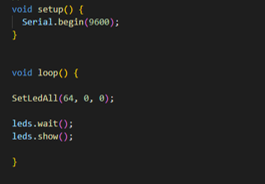
\includegraphics[width=1\textwidth]{img/015 img/Program1-červená.png}
%		\caption{Program}
%		%		\label{fig:gear-sketch2}
%	\end{minipage}
%\end{figure}


\newpage

% Návody z výkresové dokumentace
%%%% Výkresovka - textové přepisy návodů
\chapter{Výkresová dokumentace - vybrané návody}
Tato kapitola obsahuje text. přepis dvou návodů na nejběžnější operace v~sestavách.
Text je brán jako doplněk videí vypsaných v~kapitole \ref{videa-sestavy} přílohy \ref{released-videos}.

\section{Popisové pole a uživatelské vlastnosti}
Popisové pole je nedílnou součástí každého výkresu.
Udává údaje o~dané součásti, nebo sestavě, jako je označení, materiál, rozměr a podobně.
V~SolidWorks se vyplňování popisového pole řeší pomocí uživatelských vlastností, které se následně automaticky propisují na výkres.
Pro to, aby tyto vlastnosti správně fungovaly je nutné mít správně nainstalované šablony.
Jejich instalace je popsaná v~návodu \ref{instalace-sablon}.

\begin{figure}[htbp]
    \centering
    \begin{minipage}[b]{0.45\textwidth}
        \centering
        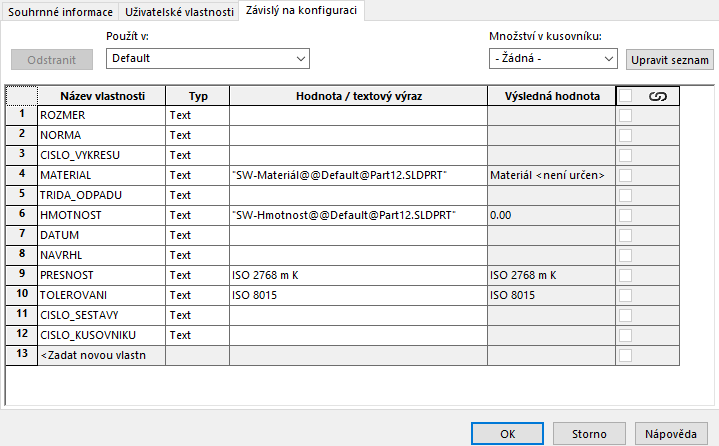
\includegraphics[width=1\textwidth]{img/030 img/vlastnosti-dilu.png}
        \caption{Tabulka vlastností souč.}
        \label{fig:realview-1}
    \end{minipage}
    \qquad
    \begin{minipage}[b]{0.45\textwidth}
        \centering
        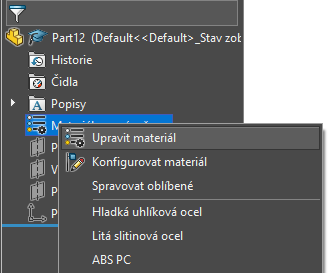
\includegraphics[width=0.7\textwidth]{img/030 img/upravit-material.png}
        \caption{Tl. pro změnu materiálu}
        \label{fig:realview-2}
    \end{minipage}
\end{figure}

Otevřeme si díl, kterému chceme upravit vlastnosti.
V~nabídce \B{Soubor} vybereme možnost \B{Vlastnosti}.
Zobrazí se nabídka vlastností dílu, ve které se musíme přepnout na kartu \B{Závislý na konfiguraci}.
Ve sloupci \B{Hodnota/textový výraz} můžeme měnit položky popisového pole.
Jakmile podle potřeby nastavíme všechny hodnoty, uložíme změny stiskem tlačítka \B{OK}.
Pro změnu kolonky \B{Materiál} musíme nastavit materiál ve Stromu FeatureManageru dané součásti.

\section{Drážka pro pero na hřídeli}
Při tvorbě výkresové dokumentace hřídele se často nevyhneme popisování drážky pro pero.
Začneme tím, že na výkres vložíme pohled hřídele tak, abychom viděli celou drážku pro pero (viz \autoref{fig:keyslot-dwg} vlevo).
Do pohledu nesmíme zapomenout přidat osu.
Na kartě \B{Výkres} vybereme \B{Řez}.
\begin{figure}[htbp]
    \centering
    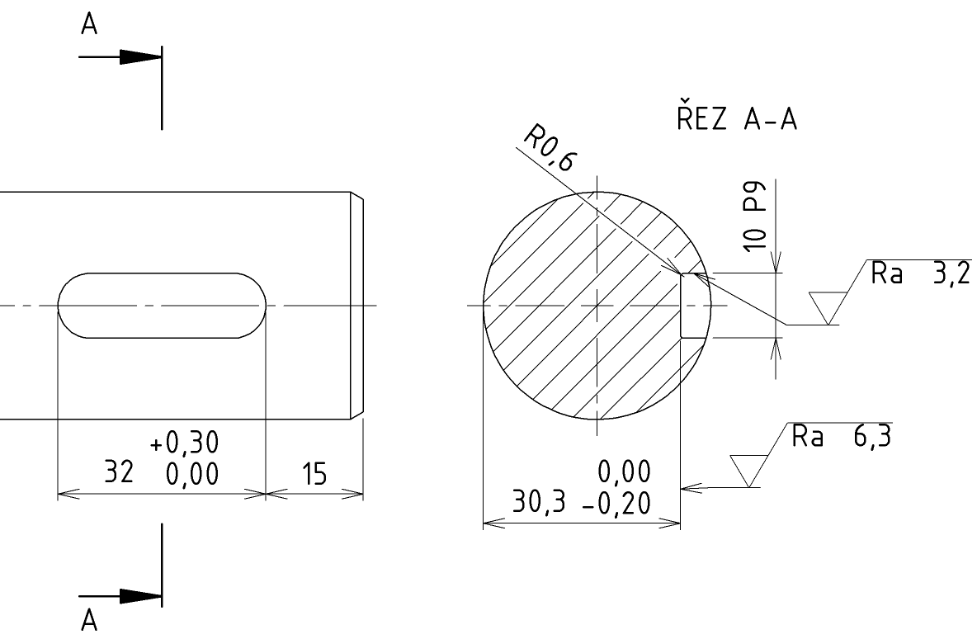
\includegraphics[width=0.65\textwidth]{img/030 img/perodrazka-hridel-screen.png}
    \caption{Popis drážky pro pero na hřídeli}
    \label{fig:keyslot-dwg}
\end{figure}

Vlevo v~nabídce nastavení řezu zvolíme svislou orientaci a řeznou čáru umístíme přibližně do středu drážky.
Zkontrolujeme si, že řez směřuje ven od středu hřídele.
Do zobrazení řezu umístíme středovou značku.

Když máme pohledy nachystané, můžeme začít popisovat.
V~pohledu zakótujeme délku drážky s~podržením klávesy \It{SHIFT} a výběrem obou krajních oblouků.
K~této kótě přidáme oboustrannou toleranci +0,3 a -0.
Dále zakótujeme vzdálenost drážky (krajního oblouku) od čela hřídele, nebo nejbližšího osazení.

Přejdeme do řezu, kde nejdříve zakótujeme šířku drážky.
Této kótě přidáme toleranci \B{P9}.
Dále zakótujeme hodnotu zaoblení dna drážky.
Posledním kótovaným rozměrem je hloubka drážky, kterou zadáme vůči protilehlému oblouku, viz \autoref{fig:keyslot-dwg} vlevo.
Zde přidáme toleranci hloubky, která je pro každou skupinu rozměrů drážek jiná -- zjistíme ji z~tabulky \ref{tab:pera-tesna}.

Posledním krokem je přidání značek drsností povrchu.
U~boků drážky se jedná o~drsnost Ra 3,2 -- značku umístíme na kótu udávající šířku drážky, viz \autoref{fig:keyslot-dwg}  vpravo.
Povrch dna drážky bude mít drsnost Ra 6,3 a umístíme jej na kótu udávající hloubku, opět viz \autoref{fig:keyslot-dwg}  vpravo.

\section{Drážka pro pero v~náboji}
Na výkres si umístíme přední pohled na náš náboj (např. ozubené kolo).
V~kartě \B{Popis} klikneme na \B{Detail}.
Střed detailního pohledu umístíme do středu díry v~náboji a jeho velikost nastavíme tak, aby byla celá drážka viditelná.
Nesmíme zapomenout přidat středové značky.
Vzhledem k~tomu, že díra s~drážkou prochází skrz náboj, její délku kótovat nemusíme.

V~zobrazení detailního pohledu ale potřebujeme zaznačit průměr díry, šířku drážky, její hloubku, velikost zaoblení, drsnosti povrchu a odpovídající tolerance.
Začneme průměrem.
Podržíme klávesu \It{SHIFT} a klikneme nejdříve na první a následně druhou stranu oblouku -- vytvoříme tak průměrovou kótu.
K~ní ještě doplníme toleranci.
Vzhledem k~tomu, že se jedná o~díru, můžeme zvolit například toleranci H7 (možné další viz \autoref{fig:jednotna-dira}).

\begin{figure}[htbp]
    \centering
    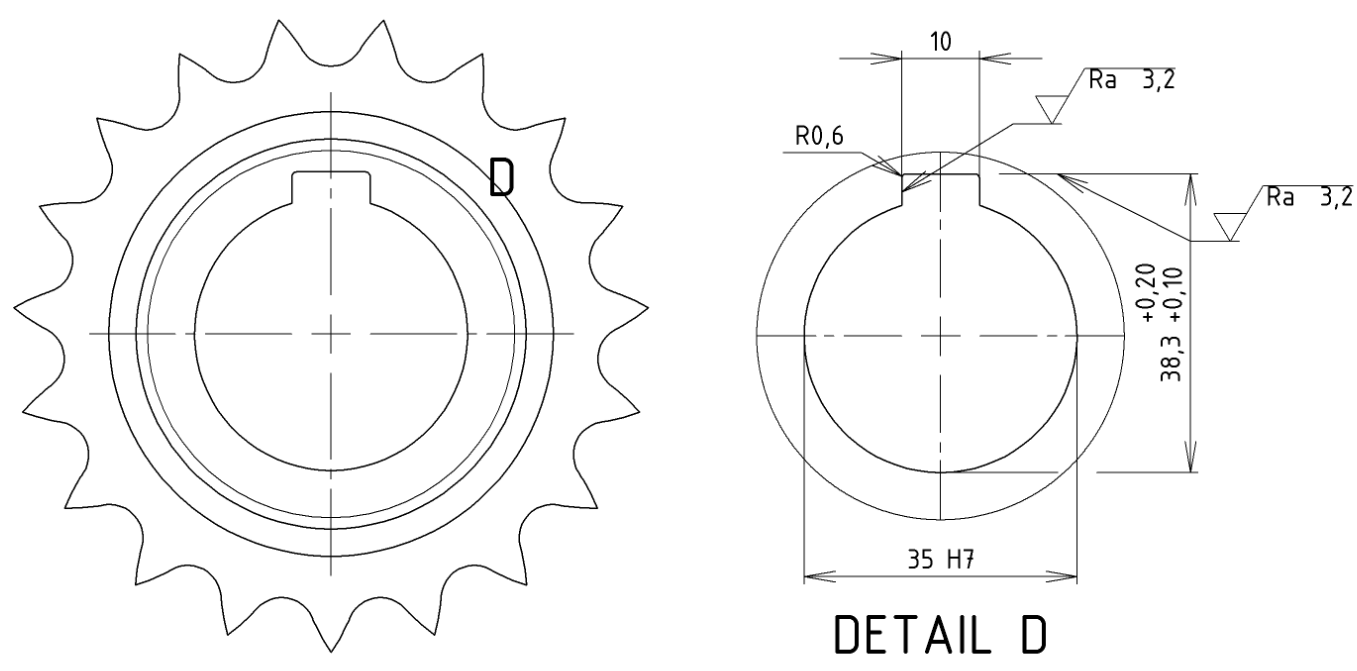
\includegraphics[width=0.6\textwidth]{img/030 img/perodrazka-naboj-screen.png}
    \caption{Plně popsaná drážka na pero v~náboji}
    \label{fig:keyhole-dwg}
\end{figure}

Po průměru musíme zakótovat šířku drážky.
Tato kóta bude mít toleranci P9, jako jsme u~drážek na pero zvyklí.
Hloubku drážky označíme stejně jako u~protikusu na hřídeli -- klikneme na hranu dna drážky, podržíme \It{SHIFT} a klikneme na protilehlý oblouk.
Ještě přidáme toleranci pro danou velikost pera -- zjistíme z~tabulky \ref{tab:pera-tesna}.
Zakótujeme zaoblení a přidáme značky drsnosti povrchu viz \autoref{fig:keyhole-dwg}.

\newpage

% Zaver prace
\chapter{Závěr}
Prototyp světla je ke dni odevzdání ročníkové práce plně funkční. Do budoucna by se dal Zkonstruovat obal, ve kterém by byla uložená elektronika (hlavně ESP-DevKit) a průhledný tvar, skrz který by LEDky zářili. Dále by se dalo vyrobit a sprovoznit těchto světel víc, a zařídit aby každé z nich bylo propojeno přes wifi s mobilem.


Tato ročníková práce mi dala hodně zabrat. Ne proto, že bych měla složité téma a nebo program by byl složitý na naprogramování, ale problém byl v tom, že jsem se musela často učit pracovat s programy a věcmi, se kterými jsem předtím nepracovala. Naučila jsem se pracovat s ESP3 a inteligentními LED světly, naučila jsem se je programovat a dokonce se napojit na ESP32-DevkitC mobilem a ovládat zařízení z mobilu.
Celkově mě ale práce na této ročníkové práci bavila a dala mi do budoucna spoustu zkušeností které se jistě budou hodit. 

\newpage

\clearpage
\phantomsection

%\appendix
%\addcontentsline{toc}{chapter}{Přílohy}

% Prilohy
%\chapter{Seznam již vydaných videí} \label{released-videos}
Tato příloha obsahuje kompletní seznam videí vzniklých v~rámci projektu P3D vč. odkazů rozdělených dle jednotlivých témat. \newline
\noindent\It{Pozn.: při kliknutí na odkaz budete přesměrování na stránku korespondujícího videa (pouze v~digitální verzi)}.

\section{Instalace a zprovoznění SolidWorks SDK} \label{videa-instalace}
\href{https://aka.parallaxproduction.cz/instalaceSDK}{Instalace a první spuštění SolidWorks SDK 2020/2021 (aka.parallaxproduction.cz/instSDK)} \newline
\href{https://aka.parallaxproduction.cz/sablony}{Instalace šablon a knihoven norm. dílů ze Sokolské (aka.parallaxproduction.cz/sablony)} \newline
\href{https://aka.parallaxproduction.cz/realview}{Aktivace Realview na necertifikované grafické kartě (aka.parallaxproduction.cz/realview)} \newline

\section{Základy modelování} \label{videa-modelovani}
\href{https://aka.parallaxproduction.cz/jednoducha-pruzina}{Jednoduchá pružina (aka.parallaxproduction.cz/jednoducha-pruzina)} \newline
\href{https://aka.parallaxproduction.cz/j-ozubene-kolo}{Ozubené kolo s~přímým čelním ozubením (aka.parallaxproduction.cz/j-ozubene-kolo)} \newline
\href{https://aka.parallaxproduction.cz/vyk-oz-kolo}{Ozubené kolo pro výkres - obálka (aka.parallaxproduction.cz/vyk-oz-kolo)} \newline
\href{https://aka.parallaxproduction.cz/jednorad-r-kolo}{Jednořadé řetězové kolo (aka.parallaxproduction.cz/jednorad-r-kolo)} \newline
\href{https://aka.parallaxproduction.cz/perodrazka-naboj}{Drážka pro pero v~náboji (aka.parallaxproduction.cz/perodrazka-naboj)} \newline
\href{https://aka.parallaxproduction.cz/perodrazka-hridel}{Drážka pro pero na hřídeli (aka.parallaxproduction.cz/perodrazka-hridel)} \newline

\section{Výkresová dokumentace} \label{videa-vykresy}
\href{https://aka.parallaxproduction.cz/popisove-pole}{Popisové pole a už. vlastnosti na výkrese (aka.parallaxproduction.cz/popisove-pole)} \newline
\href{https://aka.parallaxproduction.cz/vykres-perodrazka-na}{Výkres drážky pro pero v~náboji (aka.parallaxproduction.cz/vykres-perodrazka-hr)} \newline
\href{https://aka.parallaxproduction.cz/vykres-perodrazka-hr}{Výkres drážky pro pero na hřídeli (aka.parallaxproduction.cz/vykres-perodrazka-hr)} \newline

\section{Práce se sestavami} \label{videa-sestavy}
\href{https://aka.parallaxproduction.cz/prejmenovani-dilu}{Přejmenování dílu v~sestavě (aka.parallaxproduction.cz/prejmenovani-dilu)} \newline
\href{https://aka.parallaxproduction.cz/pack-and-go}{Přesun sestavy pomocí Pack and Go... (aka.parallaxproduction.cz/pack-and-go)} \newline

\chapter{Seznam plánovaných témat} \label{planned-videos}
V~následujícím seznamu naleznete další témata, pro která jsou videa plánována.

\subsection*{Nastavení a úpravy SolidWorks}
\begin{itemize}
    \setlength\itemsep{0.05em}
    \item Upgrade SolidWorks na novou verzi (např. 2020 na 2021),
    \item vlastní úpravy uživatelského prostředí,
    \item doplňkové moduly SolidWorks.
\end{itemize}

\subsection*{Základy modelování}
\begin{itemize}
    \setlength\itemsep{0.05em}
    \item Řetěz,
    \item řemen,
    \item plechové díly (série),
    \item svařované konstrukce (série),
    \item další normalizované prvky.
\end{itemize}

\subsection*{Výkresová dokumentace}
\begin{itemize}
    \setlength\itemsep{0.05em}
    \item Kusovník na výkrese sestavy,
    \item 
\end{itemize}

\subsection*{Sestavy}
\begin{itemize}
    \setlength\itemsep{0.05em}
    \item Základní, upřesňující a strojní vazby (série),
    \item konfigurace (pravděpodobně série).
\end{itemize}

%\chapter{Obrazové přílohy}

%\begin{figure}[h]
%    \centering
%    \includegraphics[width=0.85\textwidth]{img/ToBeRemoved/PPSB-T_BOTH.png}
%    \caption{Vizualizace PPSB-T (horní strana vpravo, dolní vlevo).}
%    \label{fig:PPSB-T_VISUAL}
%\end{figure}

\chapter{Vybrané normy}

\begin{table}[] \catcode`\-=12
    \centering
    \begin{tabular}{c|cc|c|c|c|ccccc}
    \multirow{2}{*}{\B{Průměr D}} & \multicolumn{3}{c|}{\B{Rozměr drážky}}      & \multicolumn{2}{c|}{\B{Mezní úchylky hloubky}}                                                                                              & \multicolumn{5}{c}{\B{Rozměry pera}}                                  \\ \cline{2-11} 
                                  & t   & t\subscript{1} & R\subscript{1}       & \multicolumn{1}{l|}{na hřídeli (t)}                                  & \multicolumn{1}{l|}{v náboji (t\subscript{1})}                       & b  & h  & R                     & l\subscript{min} & l\subscript{max} \\ \hline
    6 až 8                        & 1,1 & 0,9            & \multirow{2}{*}{0,2} & \multirow{4}{*}{\begin{tabular}[c]{@{}c@{}}+0,1\\ -0,0\end{tabular}} & \multirow{9}{*}{\begin{tabular}[c]{@{}c@{}}+0,2\\ +0,1\end{tabular}} & 2  & 2  & \multirow{2}{*}{0,25} & 9                & 20               \\
    8 až 10                       & 1,7 & 1,3            &                      &                                                                      &                                                                      & 3  & 3  &                       & 9                & 36               \\ \cline{1-4} \cline{7-11} 
    10 až 12                      & 2,4 & 1,6            & \multirow{4}{*}{0,4} &                                                                      &                                                                      & 4  & 4  & \multirow{4}{*}{0,5}  & 10               & 45               \\
    12 až 17                      & 2,9 & 2,1            &                      &                                                                      &                                                                      & 5  & 5  &                       & 12               & 56               \\ \cline{5-5}
    17 až 22                      & 3,5 & 2,5            &                      & \multirow{8}{*}{\begin{tabular}[c]{@{}c@{}}+0,2\\ -0,0\end{tabular}} &                                                                      & 6  & 6  &                       & 16               & 70               \\
    22 až 30                      & 4,1 & 2,9            &                      &                                                                      &                                                                      & 8  & 7  &                       & 20               & 90               \\ \cline{1-4} \cline{7-11} 
    30 až 38                      & 4,7 & 3,3            & \multirow{6}{*}{0,6} &                                                                      &                                                                      & 10 & 8  & \multirow{6}{*}{0,7}  & 25               & 110              \\
    38 až 44                      & 4,9 & 3,1            &                      &                                                                      &                                                                      & 12 & 8  &                       & 32               & 140              \\
    44 až 50                      & 5,5 & 3,5            &                      &                                                                      &                                                                      & 14 & 9  &                       & 40               & 180              \\ \cline{6-6}
    50 až 58                      & 6,2 & 3,8            &                      &                                                                      & \multirow{3}{*}{\begin{tabular}[c]{@{}c@{}}+0,4\\ +0,2\end{tabular}} & 16 & 10 &                       & 45               & 200              \\
    58 až 65                      & 6,8 & 4,2            &                      &                                                                      &                                                                      & 18 & 11 &                       & 50               & 220              \\
    65 až 75                      & 7,4 & 4,6            &                      &                                                                      &                                                                      & 20 & 12 &                       & 56               & 250             
    \end{tabular}
    \caption{Výběr z~normy ČSN 02 2562 - Pera těsná\cite{ST}}
    \label{tab:pera-tesna}
\end{table}

\begin{figure}[htbp]
    \centering
    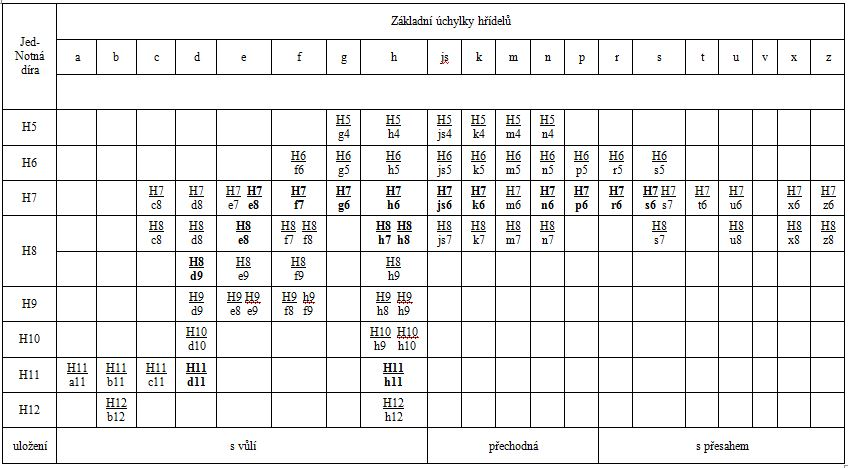
\includegraphics[width=1\textwidth]{img/jednotna-dira.JPG}
    \caption{Soustava jednotné díry, tučně zvýrazněné hodnoty jsou doporučené, převzato z~\cite{ELUC-DIRA}}
    \label{fig:jednotna-dira}
\end{figure}

\begin{figure}[htbp]
    \centering
    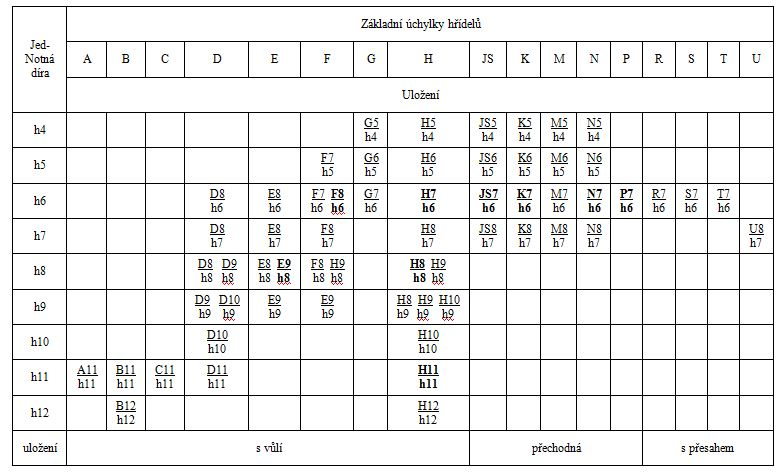
\includegraphics[width=1\textwidth]{img/jednotna-hridel.JPG}
    \caption{Soustava jednotného hřídele, tučně zvýrazněné hodnoty jsou doporučené, převzato z~\cite{ELUC-HRIDEL}}
    \label{fig:jednotna-hridel}
\end{figure}

\input literatura.tex


\listoffigures
\addcontentsline{toc}{chapter}{Seznam obrázků}

%\listoftables
%\addcontentsline{toc}{chapter}{Seznam tabulek}

\end{document}
